\documentclass{solitairemiya-art}

\title{混合随机数及其神经网络计算}
\author{李洪革（IEEE会员），陈宇豪（IEEE学生会员）}

\begin{document}

\maketitle

\begin{abstract}
随机计算（SC）的独特之处在于采用随机数（比特流）而非二进制数进行算术运算. 随机数（SN）通过CMOS门电路以伪模拟概率形式表示和携带信息. 随机数系统的再度兴起，主要与边缘计算对超低功耗和高可靠性的需求密切相关. 作为一种非位置数制表示，随机数本质上是顺序的，因而适用于某些重要的算术运算（如加/减法和乘法），并可实现超小面积电路. 本文提出一种二进制数与随机数表示相结合的新型混合数制，称为混合随机数（HSN）. 研究阐述了HSN的基本理论，并展示了混合随机计算（HSC）的特性. 基于HSC的深度神经网络硬件实现采用标准\textbf{40-nm}低功耗CMOS工艺制造，核心面积为\textbf{0.53 mm$^2$}，功耗为\textbf{102.3 mW}，时钟频率为\textbf{400 MHz}，包含4544个乘累加运算（MAC）. 

\noindent\textbf{关键词：}\songti\zihao{-4}专用集成电路（ASIC）、深度神经网络、混合随机计算（HSC）、混合随机数（HSN）、随机数. 
\end{abstract}

\section{引言}

冗余数表示的显著优势在于可使用无进位传播链进行加法运算，从而加速算术运算\cite{ref1, ref2}. 当前，硬件计算面临严格应用要求的约束，如极低成本、低功耗和高性能. 随机计算（SC）于20世纪60年代被提出，作为传统二进制数（BN）计算的低成本、低功耗替代方案\cite{ref3, ref4}. SC基于比特流的概率和均值进行计算，具有特殊性质的随机数可使用简单门电路生成，替代二进制数的复杂电路\cite{ref5, ref6}. 

二进制数在数字计算中的速度优势显著，但其算术结构需要在模块处理器之间具备较大通信宽度，以实现高性能计算系统. 在SC范式中，计算在比特流上而非二进制数上执行. 随机比特流由累积流长度中"1"出现的概率表示\cite{ref3, ref4, ref5, ref6, ref7}. SC所需的计算功率完全分布在整个低成本门电路中. 换言之，经典SC以牺牲效率为代价，通过高容错性节省大量硬件和功率资源\cite{ref3, ref7, ref8}. 尽管具备这些优势及其固有特性，SC由于高计算延迟和相对较低精度而无法取代二进制数. 高延迟本质上源于传统SC中1比特随机流的信息携带能力低下. 当随机逻辑的比特流长度等于$L$时，仅能表示$L$个不同的数据点. 显然，比特流的信息携带效率弱于二进制数. 

SC的数字计算在随机比特流上而非二进制数上执行. 为表示负数，许多SC系统采用双极性格式，使SC有效范围变为$[-1, 1]$. Gaines\cite{ref8}提出了双轨单极和双极数格式，以及每种格式的基本电路. 随机数格式已在多篇论文中讨论，在处理复杂函数的硬件利用方面具有显著优势\cite{ref9, ref10, ref11}. Alireza等人\cite{ref12}提出了一种用于单变量数学函数计算的近似混合二进制-一元计算. 一些研究者尝试使用不同技术提高SC编码效率，以解决延迟问题\cite{ref13, ref14, ref15}. 另有研究者采用确定性计算等不同技术提高SC的计算精度\cite{ref16, ref17}. Xia等人\cite{ref18}提出神经突触可塑性启发计算和可重构神经突触可塑性，用于在卷积神经网络（CNN）加速器中实现高计算效率. 总体而言，SC已被尝试应用于一系列专门领域，如神经网络\cite{ref21, ref22, ref23}、多项式计算\cite{ref19, ref20}和图像处理\cite{ref12, ref24}. 

然而，Poppelbaum\cite{ref25}观察到"短序列不可靠"，且SC的主要缺点在于低带宽导致计算速度低下. 关于随机数（SN）基本概念的一些重要理论发现尚未受到足够关注，尽管它们对SC具有积极意义. Parhi\cite{ref26}提出了分析单极、双极和混合编码格式中随机组合逻辑电路的通用方法. 使用双极和混合格式的方法可为合成任意多项式实现更简单的组合逻辑结构. Canals等人\cite{ref27}提出一种使用分数形式的新编码方法，将比特流表示的范围扩展到整个实数轴. 

为解决经典SC的固有基本问题和主要设计挑战，本文提出HSN和混合随机计算（HSC）方法，并讨论HSN表示的特性. 本研究的主要贡献如下：

\begin{enumerate}
\item 首次在二进制数或SC的数制中提出混合随机数（HSN）表示方法，融合二进制数和随机数的特性. 
\item 统一二进制数、随机数和HSN的表示，阐述三者之间的数学描述和转换关系. 
\item HSN无需二进制数与随机数之间的转换器，相比经典随机数实现了高效率和低延迟. 
\end{enumerate}

\section{数值系统}

\subsection{经典二进制数}

数表示方法随科学发展而演进. 位置数制是最传统的固定基数表示方法，其中每个位置对应的单位是其右侧相邻位置单位的恒定倍数. 数字集合为$[0, 1]$的二进制数（BN）也是一种位置数制，且为非冗余的. 它易于在CMOS逻辑电路中实现，并广泛用于中央处理器（CPU）、图形处理器（GPU）和神经网络处理单元（NPU）. 

20世纪60年代早期，Avizienis\cite{ref1}定义了一类具有对称数字集$[-\alpha, \alpha]$和基数$r > 2$的有符号数字（冗余）数制，其中$\alpha$为任意整数. 随后，研究了具有一般（可能非对称）形式$[-\alpha, \beta]$数字集的冗余有符号数字数制，作为统一实践中使用的所有冗余数表示的工具. Parhami\cite{ref2}、Gaines\cite{ref8}和Alaghi等人\cite{ref9}定义了扩展有符号数字数表示系统，新型HSN系统如图\ref{fig1}所示进行了扩展. 

\begin{figure}[htbp]
\centering
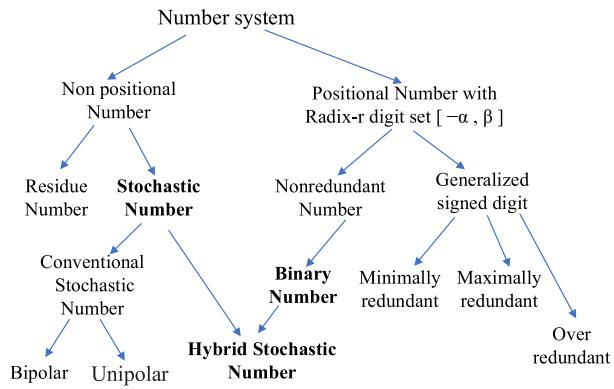
\includegraphics[width=0.8\textwidth]{images/e3e06ba8322146d442d367d9aaa15162f491de84cad2b58698c0d90911097b43.jpg}
\caption{随机数、混合随机数和经典二进制数系统}
\label{fig1}
\end{figure}

\subsection{传统随机数}

传统随机数使用单个比特流表示数据，随机比特流的期望值范围为0到1（单极性）或从$^{-1}$到1（双极性）. 本文主要关注单极性随机数. 序列中的随机数生成器（RNG）与二进制数进行比较，生成1比特编码输出，如图\ref{fig2}所示. 若二进制数大于随机数，则比较器输出高电平"1"；否则，输出低电平"0". 输出比特流的期望值等于二进制数大于随机数的概率. 当随机数为单极性形式时，比特流长度为$L$的随机数中编码1的相对频率定义为：

\begin{equation}
\hat{p} = \hat{p}(\mathrm{SN} = 1) = \frac{\sum_{j=0}^{L-1} \mathrm{SN}(j)}{L} \in [0, 1]
\end{equation}

其中$\sum_{j=0}^{L-1} \mathrm{SN}(j)$为序列中1的数量，$\hat{p}$为概率的估计值. 特定流的随机数表示并非由特定位置中单个比特的值定义，故SC属于非位置数表示. 随机数使用冗余数制，其中每个数字具有冗余表示$\hat{p}(\mathbf{SN} = \mathbf{\Omega}^{1})$. 在冗余表示中，一个代数值可用多种方式表示. 例如，对于比特流长度$L = 3$，有三种方式表示1/3：$(0, 0, 1)$、$(0, 1, 0)$和$(1, 0, 0)$. 

\begin{figure}[htbp]
\centering
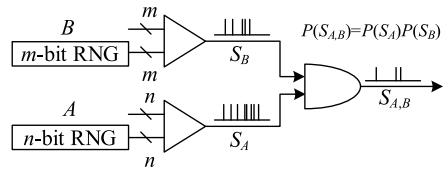
\includegraphics[width=0.6\textwidth]{images/52e336cb0a606ae2f6a2930a6ffc924c3104aee121c790e259eea49d5464daeb.jpg}
\caption{使用单极性随机比特流的随机计算}
\label{fig2}
\end{figure}

与从空间到时间编码映射相关的随机数催生了SC算术，可使用简单逻辑门电路实现. 作为另一种非位置表示，SC提高了受随机故障或元件变化影响的电路的鲁棒性. 

\subsection{随机与二进制混合数}

传统固定基数二进制数系统通常基于正整数基数（底）$r = 2$和隐式数字集$[0, 1]$. 这称为位置加权（基数）系统. 因此，

\begin{equation}
B = b_{n-1}r^{n-1} + \dots + b_1r^1 + b_0r^0 = \sum_{i=0}^{n-1} b_i \cdot r^i.
\end{equation}

\begin{definition}
考虑式(1)中随机数相对于式(2)中二进制数$B$的表示，有
\begin{equation}
\begin{aligned}
\hat{E}[S] &= \sum_{i=0}^{n-1} r^i \cdot \hat{p}(S_i = 1) = \sum_{i=0}^{n-1} r^i \left(\frac{\sum_{j=0}^{L-1} S_i(j)}{L}\right) \\
&= \frac{1}{L} \left(\sum_{j=0}^{L-1} \sum_{i=0}^{n-1} S_i(j) \cdot 2^i\right).
\end{aligned}
\end{equation}
\end{definition}

这里，$S_i$表示扩展的随机数表示，为由0-1数字流组成的二维矩阵. $S_i$的每一行形成一个随机数，$S_i$表示HSN的第$i$行. $S_i(j)$表示HSN第$i$行第$j$列的比特. $\hat{E}[S]$为HSN期望的估计值. 基于式(3)的表示系统，由多个具有不同权重的随机数组成的HSN实际上是一个二进制序列. 这种扩展的随机数表示系统称为HSN，它仍使用期望表示数据，并基于概率理论进行计算\cite{ref28, ref29}. 然而，HSN的每个比特流基于二进制数具有位置权重值，权重为$2^i$. $S$表示一个$n$比特HSN为

\begin{equation}
S = S_{n-1}2^{n-1} + \dots + S_1 2^1 + S_0 2^0
\end{equation}

其中$S_{n-1}, \ldots, S_1$和$S_0$表示基于HSN位置权重的不同随机数. $n$比特HSN的期望表示如下：

\begin{equation}
E[S] = 2^{n-1}E\left[S_{n-1}\right] + \dots + 2^1 E\left[S_1\right] + E\left[S_0\right]
\end{equation}

其中$E[S]$表示HSN不同$S_i$的期望. $n$比特HSN表示的值范围大于单个随机数，数值范围从0到$2^n - 1$. 

\begin{figure}[htbp]
\centering
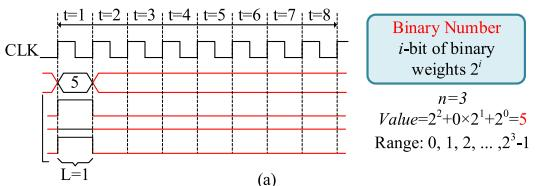
\includegraphics[width=0.3\textwidth]{images/15980863c961aa8f16ab80436ba266dd704facbfee3708c46164a318d3aceec1.jpg}\hfill
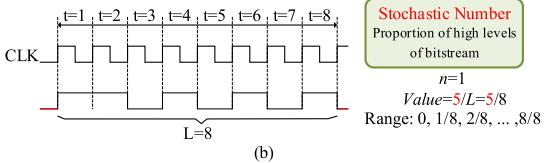
\includegraphics[width=0.3\textwidth]{images/ed35f286d6a6c9caed1bdf188d791489f22dca57dfec34d5ec7de7d57c354698.jpg}\hfill
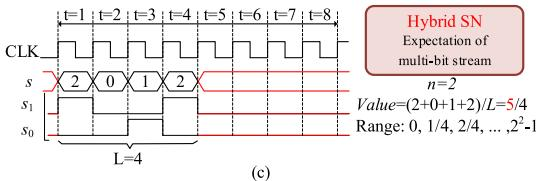
\includegraphics[width=0.3\textwidth]{images/eae01fbadf3df944e634ce8bdcc09f3c44c63c331a62bdd6e603eb6960dc33da.jpg}
\caption{(a) 二进制数、(b) 随机数和(c) 混合随机数的不同表示}
\label{fig3}
\end{figure}

\begin{example}
下面构造一个示例，从两个基本二进制序列构造基数为2的二进制序列，比特流长度$L$为16. 选择概率为$b_1$和$b_0$的基本二进制序列，使得
\[
\begin{aligned}
S &= \left[ \begin{array}{c} S_1 \\ S_0 \end{array} \right] \\
&= \left[ \begin{array}{cccc} 1\,1\,0\,1 & 1\,1\,1\,1 & 1\,1\,0\,1 & 0\,0\,1\,1 \\ 1\,0\,1\,1 & 0\,1\,0\,0 & 1\,0\,0\,1 & 1\,1\,1\,1 \end{array} \right], \quad \hat{S}_1 = b_1 = 12/16, \quad \hat{S}_0 = b_0 = 10/16.
\end{aligned}
\]

随后，从这两个流序列构造一个新的混合流（HS）序列HSN，如下所示：
\[
S = S_1 \times 2^1 + S_0 \times 2^0 = 3\,2\,1\,3\,2\,3\,2\,2\,3\,2\,0\,3\,1\,1\,3\,3
\]

\[
\begin{aligned}
\hat{E}[S] &= \frac{\sum_{j=0}^{L-1} \left[ \sum_{i=0}^{n-1} S_i(j) \cdot 2^i \right]}{L} = b_1 \times 2^1 + b_0 \times 2^0 \\
&= \frac{3 + 2 + 1 + 3 + \dots + 1 + 1 + 3 + 3}{16} \\
&= \frac{34}{16} = 2 \times \frac{12}{16} + \frac{10}{16}.
\end{aligned}
\]
\end{example}

因此，基于HSN的定义，可从一组具有二进制权重的随机数序列构造任意有限长度的HSN序列. 

\begin{definition}
观察式(3)的HSN. 
\begin{enumerate}
\item 当为二进制数时，在每个$j$处$S_i(j) = b_i$，$b_i$为0或1
\[
\hat{E}[S] = \frac{\sum_{j=0}^{L-1} [\sum_{i=0}^{n-1} S_i(j) \cdot 2^i]}{L} = \sum_{i=0}^{n-1} b_i \cdot 2^i, \text{当且仅当} n \geq 1 \text{且} L = 1.
\]

\item 当为传统随机数时
\[
\hat{E}[S] = \frac{\sum_{j=0}^{L-1} [\sum_{i=0}^{n-1} S_i(j) \cdot 2^i]}{L} = \frac{\sum_{j=0}^{L-1} S(j)}{L}, \text{当且仅当} n = 1 \text{且} L > 1.
\]

\item 当为HSN时
\[
\hat{E}[S] = \frac{\sum_{j=0}^{L-1} \left[ \sum_{i=0}^{n-1} S_i(j) \cdot 2^i \right]}{L}, \text{当且仅当} n \geq 1 \text{且} L \geq 1.
\]
\end{enumerate}
\end{definition}

随机数和二进制数的表示是HSN的两个极端，为HSN的两种特殊类型，如图\ref{fig3}所示. HSN由并行多比特流表示，遵循二进制数的位置数规则. 多比特流HSN携带的信息量或数值表示精度已显著提高. 此外，对于相同精度数表示，HSN的比特流长度$(L)$显著缩短，有效解决了传统随机数表示中的高延迟问题. 

与传统二进制数系统不同，HSN系统属于冗余数表示. 使用HSN对同一数字编码可能产生多种表示，类似于随机数. 例如，$(2, 0, 1, 2)_{\mathrm{HSN}}$、$(2, 1, 1, 1)_{\mathrm{HSN}}$和$(1, 3, 1, 0)_{\mathrm{HSN}}$具有相同值，因为三个HSN的均值均等于5/4. 因此，HSN系统是冗余数系统的代表. 

\begin{example}
将二进制数$x$编码为HSN. 第一步将$x$拆分为$n$个具有较小比特宽度的二进制数，$\mathrm{BN}_0, \mathrm{BN}_1, \ldots, \mathrm{BN}_{n-1}$. $x$与$\mathrm{BN}_i$之间的关系描述如下：
\begin{equation}
x = \mathrm{BN}_{n-1}2^{n-1} + \dots + \mathrm{BN}_1 2^1 + \mathrm{BN}_0 2^0.
\end{equation}

$\mathrm{BN}_i$的比特宽度为$k_i$，$k_i \in \mathbb{N}^+$. 第二步将$\mathbf{BN}_0, \dots, \mathbf{BN}_{n-1}$编码为随机数. 它们与$k_{\mathrm{max}}$比特RNG进行比较. 因此，$n$个随机数的期望携带相同系数$2^{-k_{\mathrm{max}}}$. $k_{\mathrm{max}}$为$k_i$的最大值
\begin{equation}
\left\{ \begin{array}{ll}
\text{if } \mathrm{BN}_i > \mathrm{RNG}(j), & S_i(j) = 1 \\
\text{else} & S_i(j) = 0
\end{array} \right.
E[S_i] = \mathrm{BN}_i / 2^{k_{\max}} \quad (i = 0, 1, \dots, n-1).
\end{equation}
\end{example}

\begin{definition}
结合式(4)--(7)，HSN的期望可表示为：
\begin{equation}
E[S] = \sum_{i=0}^{n-1} 2^i E[S_i] = \frac{\sum_{i=0}^{n-1} 2^i \mathrm{BN}_i}{2^{k_{\max}}} = \frac{x}{2^{k_{\max}}}.
\end{equation}
\end{definition}

HSN输出成功表示$x$，其期望具有系数$2^{-k_{\mathrm{max}}}$. 图\ref{fig4}(a)提供了一个3比特HSN生成示例，以解释编码电路的细节. 

\begin{figure}[htbp]
\centering
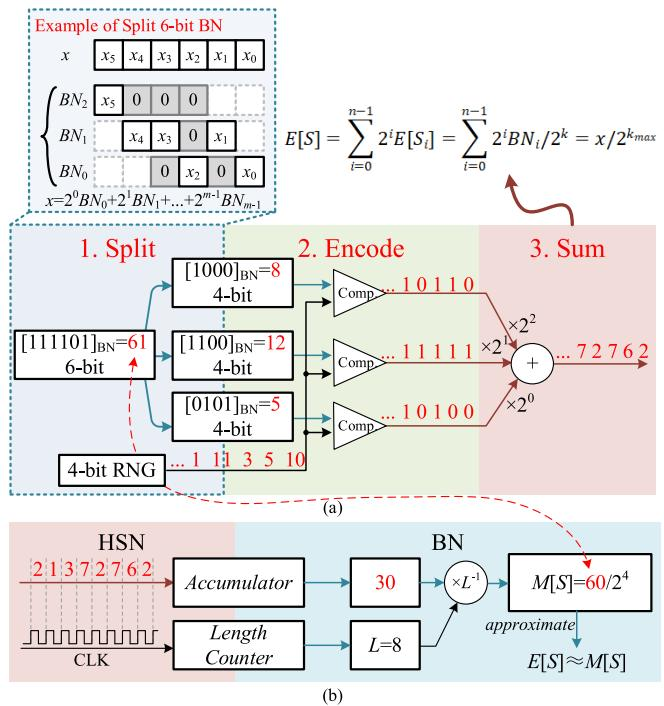
\includegraphics[width=0.9\textwidth]{images/a41eb1dcafacd892093e122c089913564e97f0795027787e55c9af974160fcac.jpg}
\caption{HSN的编码和解码过程. (a) 6比特二进制数被编码为3比特HSN. (b) HSN被解码为二进制数. }
\label{fig4}
\end{figure}

如前所述，HSN表示的值由其期望确定，期望通过计算无限长度HSN的均值获得，这在实际电路中不可实现. 因此，计算有限长度流的HSN均值以获得近似期望，如图\ref{fig4}(b)所示

\begin{equation}
E[S] = \lim_{L \to \infty} M[S] = \lim_{L \to \infty} \sum_{t=1}^{L} S(t) / L
\end{equation}

其中$M[S]$表示$S$的均值，$s$为HSN. 为便于区分HSN中的行和列，$S(t)$表示$S$中第$t$列组成的数字. 此操作可使用累加器和计数器实现. 累加器用于计算$\sum_{t=1}^{L} S(t)$，计数器用于计算比特流长度$L$. 当$L = 2^n, n \in \mathbb{N}$时，除法可用移位代替. 

\subsection{HSC的算术运算}

\subsubsection{乘法}

最常见的情况是两个HSN的乘法，如\cite{ref29}中所讨论的. $S_a$和$S_b$表示两个HSN，比特流长度均为$L$. 在HSC中，$S_c$的期望等于$S_a$期望与$S_b$期望的乘积. 乘法运算输入和输出期望之间的关系表示为式(10). 当$S_a$和$S_b$独立时，实现乘法运算

\begin{equation}
\begin{aligned}
E[S_c] &= E[S_a \cdot S_b] \\
&= E\left[S_a\right] \cdot E\left[S_b\right] \text{ 当且仅当 } S_a, S_b \text{ 独立. }
\end{aligned}
\end{equation}

此类乘法可能产生误差，主要原因有两方面. 首先，输入之间很难实现完全独立的关系. 其次，使用有限长度HSN的均值近似HSN的期望可能产生误差. 图\ref{fig5}(a)展示了这种方法的一个示例. 在此示例中，输出HSN的均值没有误差. 然而，这种情况是特例，误差并不总是0. 

假设$S_a$和$S_b$分别为$n$比特和$m$比特HSN. 将式(10)更改为随机数的位置加权格式，获得HSN的$S_c$表达式

\begin{equation}
\begin{aligned}
E\left[S_c\right] &= E\left[S_a \cdot S_b\right] \\
&= E\left[\left(\sum_{i=0}^{n-1} 2^i S_{a,i}\right) \left(\sum_{j=0}^{m-1} 2^j S_{b,j}\right)\right] \\
&= \sum_{i=0}^{n-1} \sum_{j=0}^{m-1} 2^{i+j} E\left[S_{a,i} \cdot S_{b,j}\right]
\end{aligned}
\end{equation}

\begin{equation}
\begin{aligned}
E\left[S_c\right] &= \sum_{i=0}^{n-1} \sum_{j=0}^{m-1} 2^{i+j} E\left[S_{a,i}\right] \cdot E\left[S_{b,j}\right] \\
&= E\left[S_a\right] \cdot E\left[S_b\right] \text{ 当且仅当 } S_{a,i}, S_{b,j} \text{ 独立. }
\end{aligned}
\end{equation}

$S_{a,i}$表示$S_a$中权重为$2^i$的第$i$个随机数，$S_{b,j}$类似. 从式(11)的期望表达式来看，只有当两个随机数位于不同HSN中时，它们才相乘，故需要独立. 独立性要求可使用现有方案解决，如Sobol序列\cite{ref12}或独立RNG等. 至于同一HSN中的两个随机数，它们之间没有乘法，故无独立性要求. 因此，允许同一HSN中的二进制数到随机数编码使用相同的RNG，这不违反乘法运算的独立性要求. 

作为式(3)中HSN的概念，二进制数可看作常数HSN. 基于期望的性质，当其中一个输入被常数HSC替换时，无条件建立$E[S_a \cdot S_b] = E[S_a] \cdot E[S_b]$. 因此，它不需要乘法的独立性要求，且操作精度不会因非独立输入而受影响. 图\ref{fig5}(b)展示了$m$比特二进制数$x$和$n$比特HSN$S_a$乘法的示例. 输出是$(m+n)$比特HSN，其比特宽度由输入二进制数和HSN的比特宽度确定. 无条件实现乘法的输出HSN的期望和均值如下：

\begin{figure}[htbp]
\centering
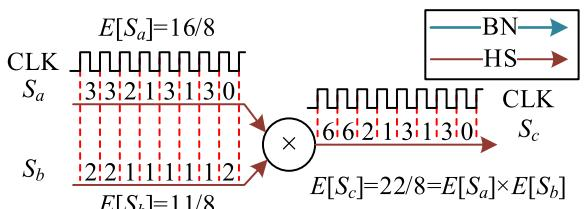
\includegraphics[width=0.48\textwidth]{images/da7115a83654b080e87b7bf275cd06acd979bb925e8982fe638b667f43c8de05.jpg}\hfill
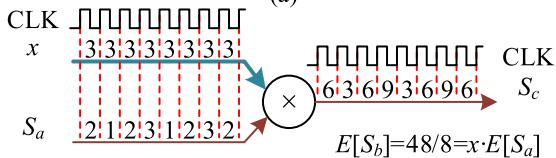
\includegraphics[width=0.48\textwidth]{images/825de683637bbb9175e53f6df5a6fef86793e6d1fba60ed93e98cfafb61680fd.jpg}
\caption{HSC不同输入类型的乘法方法. (a) $\mathrm{HSN} \times \mathrm{HSN}$和(b) $\mathrm{BN} \times \mathrm{SN}$，输出比特宽度可变. }
\label{fig5}
\end{figure}

\begin{equation}
M\left[S_c\right] = \sum_{t=1}^{L} x \cdot S_a(t) / L = x \cdot M\left[S_a\right]
\end{equation}

\begin{equation}
E\left[S_c\right] = E\left[x \cdot S_a\right] = x \cdot E\left[S_a\right].
\end{equation}

在HSC域中，非独立输入不会影响计算. 计算误差仅由HSN的编码精度引起，即$S_a$的均值与其期望之间的差异. 当$n$比特二进制数到$m$比特HSN的流$L$增加到$2^{n+m-1}$时，编码误差为0. 

因此，其均值完全等于期望，$\mathrm{HSN} \times \mathrm{BN}$的计算完全准确. 低差异序列可用作HSC中的随机源，这在编码精度方面带来好处. 当然，经典SC方案中的普通LFSR或计数器也可在HSC中工作. 由于随机源对整个乘法精度的影响仅在于二进制数到HSN编码的步骤，当$L$较小时，低差异序列比其他序列具有更好的精度. 众所周知，确定性系统可以实现完全准确的计算. HSC的计算操作也是如此，即二进制数到HSN的转换过程中没有误差. 因此，HSC可以像确定性系统一样实现完全准确的计算. 此外，HSC通过多比特并行编码实现更高效率，在计算延迟方面具有显著优势. 

\subsubsection{加法和减法}

HSC加法器在算术运算中通过缩放加法实现，它由$n$个MUX与$n$比特HSN组成. 或者可使用二进制加法器实现加法，如图\ref{fig6}(b)和(c)所示. 类似于HSC的乘法，使用三种格式类型的输入，输出为HSN. 

常见的情况是输入为两个HSN. $S_a$和$S_b$为加法的两个输入，流长度均为$L$. $S_c$为HSC输出的期望，等于输入$S_a$和$S_b$期望之和. 这是通过将$S_a$和$S_b$中对应的数字相加实现的\cite{ref29}. 减法运算与加法相同，这两种运算在式(14)中描述. 输出的期望和均值如下式所示：

\begin{equation}
E\left[S_c\right] = E\left[S_a \pm S_b\right] = E\left[S_a\right] \pm E\left[S_b\right]
\end{equation}

\begin{equation}
M\left[S_c\right] = \frac{\sum_{t=1}^{L} \left[S_a(t) \pm S_b(t)\right]}{L} = M\left[S_a\right] \pm M\left[S_b\right].
\end{equation}

这里，流长度$t$从1到$L$取每个整数值，生成$S_c(1), S_c(2), \ldots, S_c(L)$. 在有符号HSN中，允许包括负的$S(t_i)$和正的$S(t_j)$的情况，且$t_i \neq t_j$. 

\begin{figure}[htbp]
\centering
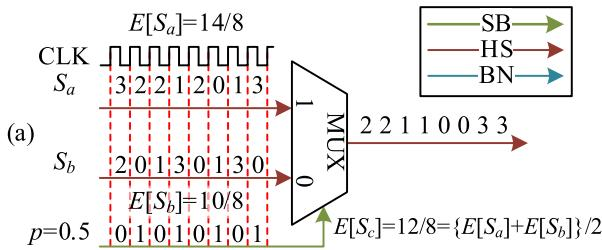
\includegraphics[width=0.32\textwidth]{images/6c627216633d899d73c7601e7fdab1d72f216c1932a3bbcd8ecf3296238e5384.jpg}\hfill
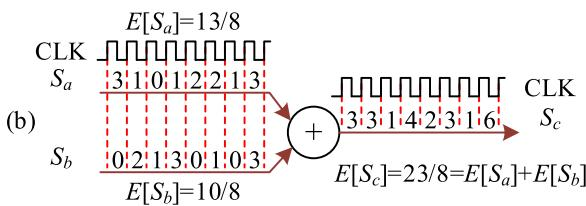
\includegraphics[width=0.32\textwidth]{images/a4a6a6bbcd6285c1a39d554a16e6307d7c035775c4b2b58c94262baa9f0acf07.jpg}\hfill
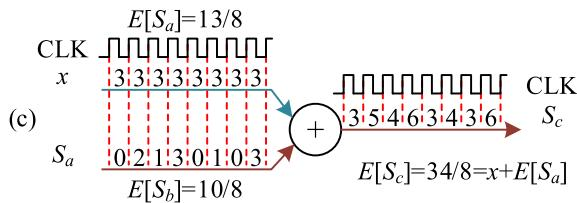
\includegraphics[width=0.32\textwidth]{images/3dd51fc3f522bbde66bb534bfce710691c63bba5cb6ae4ff3ff4fc5a99219033.jpg}
\caption{加法允许二进制数、随机数或HSN作为输入. (a) 使用MUX（多路选择器）的缩放加法，(b) 两个HSN输入的HSC加法器，和(c) 二进制数和HSN两个输入的HSC加法器. }
\label{fig6}
\end{figure}

\section{HSC的神经网络实现}

\subsection{激活函数逼近}

激活函数的计算电路以逐次逼近形式设计. HSC中的函数计算要求输入和输出的期望（$E_{\mathrm{in}}$和$E_{\mathrm{out}}$）满足函数关系，即$E_{\mathrm{out}} = f(E_{\mathrm{in}})$. 然而，HSC的长度是有限的. 因此，它使用HSN的均值代替期望，即输入和输出（$M_{\mathrm{in}}$和$M_{\mathrm{out}}$）满足$M_{\mathrm{out}} = f(M_{\mathrm{in}})$. $S(t)$表示时间$t$时的HSN数字$s$，式(16)展示了$S(t)$、均值$(M)$和总和（Sum）之间的关系. $L$为$S(t)$的流长度，$t = 1, 2, \ldots, L$

\begin{equation}
\mathrm{Sum} = \sum_{t=1}^{L} S(t) = M \cdot L.
\end{equation}

根据式(16)，$M_{\mathrm{in}}$和$M_{\mathrm{out}}$之间的函数关系可转换为$\mathrm{Sum}_{\mathrm{in}}$和$\mathrm{Sum}_{\mathrm{out}}$的函数，如下式所示：

\begin{equation}
M_{\mathrm{out}} = \frac{\mathrm{Sum}_{\mathrm{out}}}{L} = f\left(\frac{\mathrm{Sum}_{\mathrm{in}}}{L}\right) = f(M_{\mathrm{in}}).
\end{equation}

因此，获得了$\mathrm{Sum}_{\mathrm{in}}$和$\mathrm{Sum}_{\mathrm{out}}$之间的关系. 函数$g(x)$是$f(x)$的拉伸变换，如下所示：

\begin{equation}
\mathrm{Sum}_{\mathrm{out}} = g(\mathrm{Sum}_{\mathrm{in}}) = L \cdot f\left(\frac{\mathrm{Sum}_{\mathrm{in}}}{L}\right).
\end{equation}

当$L$接近无穷大时，式(17)变化如下：

\begin{equation}
\begin{aligned}
E_{\mathrm{out}} &= \lim_{L \to \infty}(M_{\mathrm{out}}) = \lim_{L \to \infty} \frac{g(\mathrm{Sum}_{\mathrm{in}})}{L} \\
&= f\left(\lim_{L \to \infty} \frac{\mathrm{Sum}_{\mathrm{in}}}{L}\right) = f(E_{\mathrm{in}}).
\end{aligned}
\end{equation}

为实现上述关系$\mathrm{Sum}_{\mathrm{out}} = g(\mathrm{Sum}_{\mathrm{in}})$，并根据式(20)获得输出HSN，这是逐次逼近的过程，如图\ref{fig7}(a)所示

\begin{equation}
S_{\mathrm{out}}(t) = \left\{ \begin{array}{ll}
g[S_{\mathrm{in}}(1)], & t = 1 \\
g\left[\sum_{\tau=1}^{t} S_{\mathrm{in}}(\tau)\right] - \sum_{\tau=1}^{t-1} S_{\mathrm{out}}(\tau), & t > 1.
\end{array} \right.
\end{equation}

然后使用以下方程获得HSC输出的总和，实现函数计算：

\begin{equation}
\begin{aligned}
\mathrm{Sum}_{\mathrm{out}} &= \sum_{\tau=1}^{L} S_{\mathrm{out}}(\tau) \\
&= g\left[\sum_{\tau=1}^{L} S_{\mathrm{in}}(\tau)\right] = g(\mathrm{Sum}_{\mathrm{in}}).
\end{aligned}
\end{equation}

\begin{figure}[htbp]
\centering
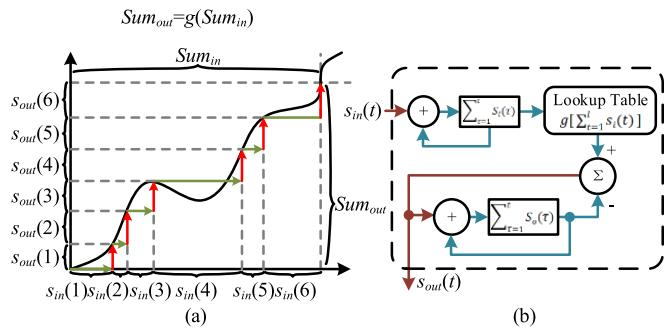
\includegraphics[width=0.9\textwidth]{images/5bbd3f278f20dc8ca76283de85ae8d6b1b5164ac71bea6dce12d952425866b37.jpg}
\caption{使用逐次逼近方法实现的函数计算. (a) 逐次逼近过程示例. (b) 逐次逼近方法电路. }
\label{fig7}
\end{figure}

电路如图\ref{fig7}(b)所示. $S_i(t)$由累加器接收以获得$\sum_{\tau=1}^{t} S_i(\tau)$. 函数计算$g(x)$可使用可以拟合任何函数的查找表（LUT）实现. $g(x)$根据式(18)从原始函数$f(x)$获得. 当Relu()的输出为$S_{\mathrm{out}}(t)$时，Reg2累加器同时接收$S_{\mathrm{out}}(t)$以获得$\sum_{\tau=1}^{t} S_{\mathrm{out}}(\tau)$. 

Relu()函数是神经网络的常见激活函数. 它使用逐次逼近方法实现. 图\ref{fig7}(b)中所示的LUT可被图\ref{fig8}中的正负数判断电路替代，这降低了硬件成本. LeakyRelu()也可不使用LUT实现. 区别是MUX的port0输入为$a\sum_{\tau=1}^{t} S_{\mathrm{in}}(\tau)$而非0，$a$为LeakyRelu()的常数系数. 为简化电路，建议$a$为$2^{-k}, k \in \mathbb{Z}$，乘法可使用移位操作实现. 

\begin{figure}[htbp]
\centering
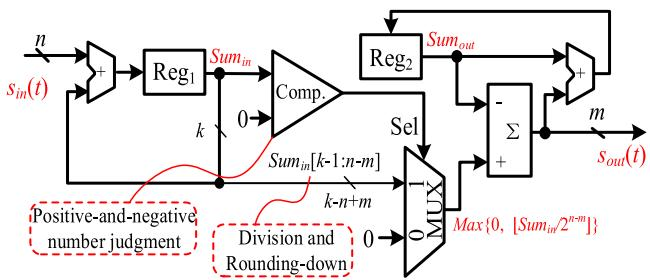
\includegraphics[width=0.7\textwidth]{images/f690d941e618429b44a37c55e713ff1b51e9f80636db18f8a73d0c7528fdbc56.jpg}
\caption{使用逐次逼近方法实现的Relu()函数电路. }
\label{fig8}
\end{figure}

此外，HSN的输出可被截断以减少比特宽度. 以图\ref{fig8}中的Relu()为例，HSC的输入比特宽度为$n$比特. 为获得$m$比特输出HSN，式(20)和(21)的激活函数被以下方程替代：

\begin{equation}
\begin{aligned}
\mathrm{Sum}_{\mathrm{out}} &= \sum_{\tau=1}^{L} S_{\mathrm{out}}(\tau) \\
&= \left\lfloor \frac{g\left[\sum_{\tau=1}^{L} S_{\mathrm{in}}(\tau)\right]}{2^{n-m}} \right\rfloor = \left\lfloor \frac{g(\mathrm{Sum}_{\mathrm{in}})}{2^{n-m}} \right\rfloor
\end{aligned}
\end{equation}

\begin{equation}
S_{\mathrm{out}}(t) = \left\{ \begin{array}{ll}
\left\lfloor \frac{g[S_{\mathrm{in}}(1)]}{2^{n-m}} \right\rfloor, & t = 1 \\
\left\lfloor \frac{g\left[\sum_{\tau=1}^{t} S_{\mathrm{in}}(\tau)\right]}{2^{n-m}} \right\rfloor - \sum_{\tau=1}^{t-1} S_{\mathrm{out}}(\tau), & t > 1
\end{array} \right.
\end{equation}

其中$\lfloor \cdot \rfloor$表示向下取整操作. 一般而言，截断应在Relu()操作之后进行，如式(22)所示. 然而，在图\ref{fig8}中，它在Relu()操作之前进行. 此调整是为了减少MUX的输入比特宽度，对计算结果没有影响，这是Relu()或LeakyRelu()的特殊设计. 当计算其他复杂函数时，复杂函数也可基于式(22)和(23)截断输出HSN. 该方案可灵活调整输出HSN的比特宽度，有助于减少下一级级联电路的硬件开销. 

\subsection{神经元电路}

在传统SC中，数据必须在随机数和二进制数之间反复转换，以避免独立性的影响. 因此，电路很难实现流水线架构，数据转换需要大量处理时间，导致高延迟. 因此，从计算效率来看，即每焦耳（或每面积）每秒的操作数，由于信息效率和编码成本的巨大劣势，现实中SC的能量（或面积）效率通常比传统二进制计算更差. SC的低成本优势尚未得到充分利用. 本文提出的HSC解决了这个问题，数据不再需要在不同格式之间转换，从而节省了转换的时间成本和硬件开销. HSC方法可在大规模并行和复杂计算情况下展示其优势，如神经网络. 

\begin{figure}[htbp]
\centering
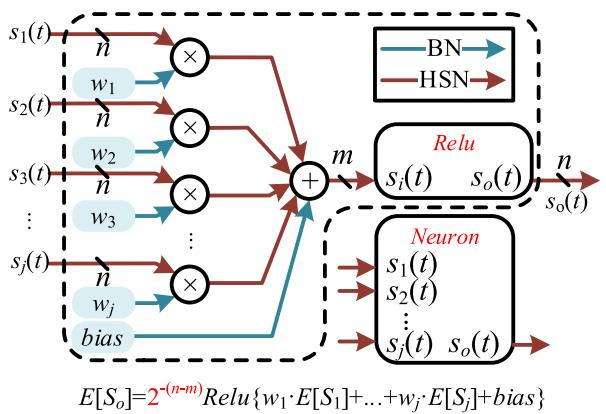
\includegraphics[width=0.9\textwidth]{images/d2fcef0388262d1fc7249c6e8f632c7b0ca218913bbb45029a7ccfc3101eebd1.jpg}
\caption{基于HSC的神经元结构，无需权重和偏置数据的任何转换器. 输入和输出是HSN，输出HSN的比特宽度可以调整. }
\label{fig9}
\end{figure}

神经元电路基于HSC设计，如图\ref{fig9}所示. 在设计中使用二进制加法器作为HSC加法器. 虽然二进制加法器比MUX加法器占用更大面积，但它可实现更高计算精度和更低延迟. $S_1(t), S_2(t), \ldots, S_i(t)$为表示神经元输入的$n$比特HS，$w_1, w_2, \ldots, w_j$和偏置为存储为二进制数的神经元参数. 神经元使用Relu()作为激活函数，如图\ref{fig8}所示. Relu()还执行截断以确保输入和输出HSN具有相同比特宽度. 输入和输出HS使用相同比特宽度以实现多个神经元的级联连接. 因此，可形成神经网络的流水线架构以实现低延迟性能. 此外，传统SC的数据转换问题，即随机数和二进制数之间的重复转换，也得到了解决. 

\begin{table}[htbp]
\centering
\caption{不同突触数量神经元电路的硬件结果}
\label{tab1}
\begin{tabular}{cccccccc}
\toprule
突触数量 & \multicolumn{2}{c}{方法} & LUT & FF & 功耗(W) & 每突触功耗(mW) & L. \\
\midrule
\multirow{3}{*}{32} & \multirow{2}{*}{HSC} & 1-bit & 388 & 344 & 0.02 & 0.63 & 256 \\
 & & 2-bit & 631 & 453 & 0.031 & 0.97 & 128 \\
 & \multicolumn{2}{c}{B.(8-bit)} & 3142 & 1065 & 0.105 & 3.28 & 1 \\
\midrule
\multirow{3}{*}{64} & \multirow{2}{*}{HSC} & 1-bit & 736 & 667 & 0.036 & 0.56 & 256 \\
 & & 2-bit & 951 & 786 & 0.046 & 0.72 & 128 \\
 & \multicolumn{2}{c}{B.(8-bit)} & 6249 & 2151 & 0.21 & 3.28 & 1 \\
\bottomrule
\end{tabular}
\\[0.5em]
\small
所有数据均从FPGA配套设计套件KCU116获得. 时钟频率为300 MHz. 输入HSC的比特宽度为1比特或2比特. 权重和偏置为8比特二进制数. 二进制电路由设计套件自动优化. B.表示二进制，L.表示延迟. 
\end{table}

表\ref{tab1}显示了基于HSC和传统二进制的不同突触数量神经元电路的实现结果，其中HSC的电路按照图\ref{fig9}实现. $S_i(t)$设置为1比特HSN，$w_j$和偏置设置为8比特有符号二进制数. 随着突触数量的增加，Relu()电路的成本被平均到每个突触. 因此，64输入情况下的平均功耗略低于32输入. HSC（1比特HSN）实现的神经元的硬件需求不到二进制实现神经元的$20\%$. 随着比特宽度的增加，HSC的硬件成本优势可进一步扩大. 网络参数直接存储在计算单元附近，无需从外部存储器重复读取数据. 因此，它避免了二进制人工智能（AI）加速器速度受数据调度速度限制的问题. 

\subsection{神经网络应用}

基于图\ref{fig9}所示的神经元电路，构建了一个五层全连接神经网络，用于分类两个线性不可分的半月形数据. 深度网络的结构为$[2, 64, 32, 32, 32, 2]$. 分类结果如图\ref{fig10}所示. 使用软件（PyTorch和MATLAB）进行深度网络训练. 网络的权重和偏置，包括输入$x$和$y$，均经过8比特量化. 二分类的边界由图\ref{fig10}中的红色虚线表示. 基于不同流长度的HSC的分类边界用不同颜色的实线绘制. 当$L \geq 2^6$时，HSC与二进制之间边界的差异仍然很小. 即使$L$降低到$2^5$，从HSC获得的边界也能清楚地区分两组点. 

\begin{figure}[htbp]
\centering
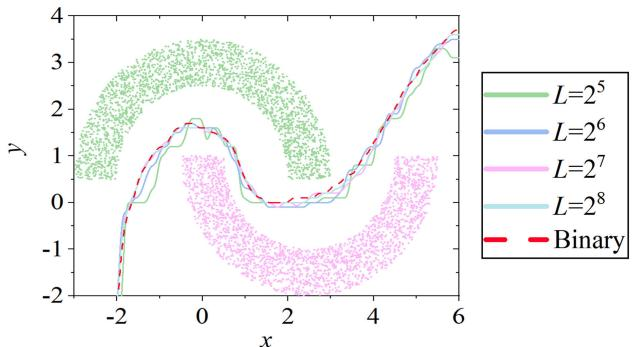
\includegraphics[width=0.7\textwidth]{images/0daa35219931db586f72b52c45e478d252ff62b0aa22b3875a202ea3be89c949.jpg}
\caption{使用深度网络对两个线性不可分半月形数据进行分类；$L$是流长度. }
\label{fig10}
\end{figure}

\begin{table}[htbp]
\centering
\caption{基于FPGA的深度神经网络硬件实现}
\label{tab2}
\begin{tabular}{cccc}
\toprule
量化比特宽度 & LUT & FF & 功耗(W) \\
\midrule
8-bit & 53110 & 47503 & 2.389 \\
\midrule
突触数量 & 时钟频率(MHz) & 计算性能(TOPS) & 能效(TOPS/W) \\
\midrule
4544 & 300 & 2.726/L & 1.141/L \\
\bottomrule
\end{tabular}
\\[0.5em]
\small
所有数据均从FPGA配套设计套件KCU116获得. $L$表示HSC的比特流长度. 
\end{table}

使用硬件电路验证了基于HSC的该神经网络. 基于HSC的网络的主要特点是多次乘法时输入数据的非独立性，而非传统SC的独立性要求. 测试中的网络包含4544个突触，由4544个乘累加（MAC）组成. 实现结果如表\ref{tab2}所示. 乘法器和加法器的平均硬件规模仅为11.7 LUTs和10.5 FFs. 在300 MHz时钟下，它可在2.389 W功率下每秒执行$2.726 \times 10^{12}$次HSC操作（OPS），相当于$2.726/L \times 10^{12}$二进制OPS. $L$为比特流长度，取决于精度要求. 

上述基于HSC的全连接（FC）神经网络使用40-nm CMOS技术实现和制造. 深度神经网络的结构设置为$[64, 32, 32, 32, 10]$，用于MNIST分类. 使用PyTorch进行网络训练. 因为照片从$28 \times 28$调整为$8 \times 8$以减少MAC数量，使用浮点数在软件中的误分类率增加到$3.89\%$. 基于范围线性对称量化方法，网络的权重和偏置以及输入数据通过MATLAB量化为8比特INT，误分类率为$3.96\%$. 

\begin{figure}[htbp]
\centering
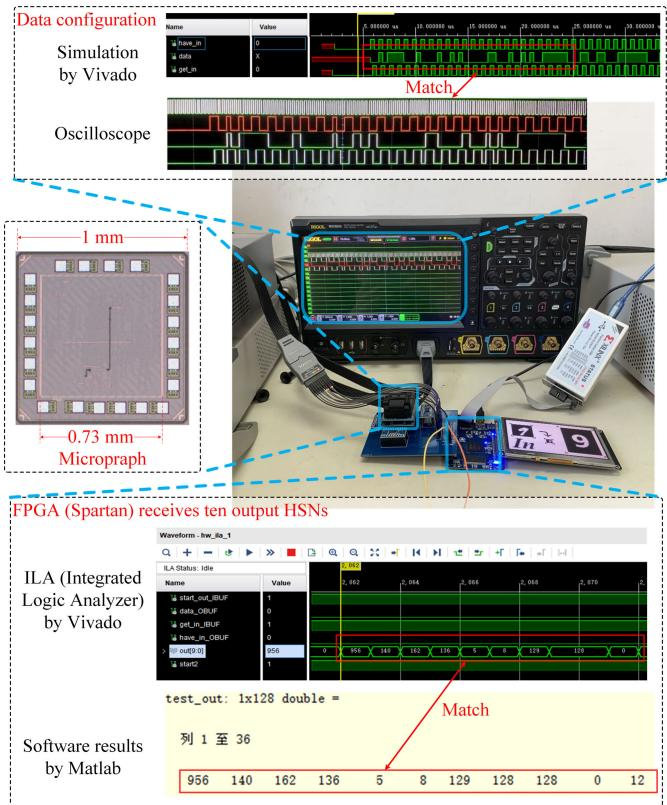
\includegraphics[width=0.9\textwidth]{images/3b7674bf4cc1bdc97522877d6c33653171392349c6b712393ae1dc848008b244.jpg}
\caption{基于HSC的神经网络的芯片显微照片和数字识别实验. 当$L = 32$时，MNIST上的准确率达到$96.01\%$. 照片调整为$8 \times 8$以减少MAC数量. }
\label{fig11}
\end{figure}

神经网络的芯片显微照片如图\ref{fig11}所示，其中芯片面积为$1.0 \, \mathrm{mm}^2$，神经网络的核心面积仅为$0.73 \times 0.73 \, \mathrm{mm}^2$. 网络结构由4544个乘累加（MAC）组成，专用集成电路（ASIC）的实现结果如表\ref{tab3}所示. 表\ref{tab3}列出了几种基于SC或二进制的设计. 传统SC设计\cite{ref30, ref31, ref32}受长比特流长度劣势的限制，其能效低于ASIC实现的二进制设计. 使用流水线架构的设计\cite{ref33}表现出高能效. 使用模拟电路实现SC的设计\cite{ref34}显著提高了能效；然而，其网络仅第一层使用SC实现. 当基于ASIC实现HSC网络时，它可在400 MHz时钟下以102.3 mW功率执行$3.635 \times 10^{12}$次HSC OPS（$3.635 \times 10^{12}/L = 1.136 \times 10^{11}$二进制OPS）. 一个$\mathrm{SOPS} = 1/L$ OPS，其中$L$为比特流长度，取决于精度要求. 面积效率为$6.82 \, \mathrm{TSOPS}/\mathrm{mm}^2$，能效为142.6--35.53 TSOPS/W（这里$L = 8$--32）. HSC神经网络（$L = 32$）的能效是传统SC设计的50倍以上，这与模拟或二进制神经网络设计的性能相似. 与8比特整数神经网络相比，基于HSC的网络在Top-1精度上损失很小，仅下降$0.03\%$，从$96.01\%$降至$96.04\%$. 受益于神经网络的鲁棒性，计算精度上的小牺牲对推理精度影响很小. 而且，之前的作品\cite{ref30, ref31, ref32, ref33, ref34}也证实了这一点，这些SC设计都取得了良好的推理精度. 当比特流长度$L$压缩到8时，神经网络的能效可比$L = 32$时提高四倍，尽管误分类率将增加到$11.3\%$. 

\begin{table*}[htbp]
\centering
\caption{与其他神经网络设计的比较}
\label{tab3}
\resizebox{\textwidth}{!}{%
\begin{tabular}{cccccccccccccc}
\toprule
\multirow{3}{*}{方法} & \multicolumn{5}{c}{SC} & \multicolumn{4}{c}{BN} & \multicolumn{3}{c}{\multirow{3}{*}{本文提出的HSC(8-BIT)}} \\
\cmidrule(lr){2-6} \cmidrule(lr){7-10}
 & \multicolumn{3}{c}{传统} & 流水线 & 模拟 & \multicolumn{2}{c}{16-bit} & \multicolumn{2}{c}{8-bit} & & & \\
\cmidrule(lr){2-4} \cmidrule(lr){5-5} \cmidrule(lr){6-6} \cmidrule(lr){7-8} \cmidrule(lr){9-10}
 & \cite{ref30} & \cite{ref31} & \cite{ref32} & \cite{ref33} & \cite{ref34} & \cite{ref35} & \cite{ref36} & \cite{ref37} & \cite{ref38} & & & \\
\midrule
工艺 & ASIC45nm & ASIC45nm & ASIC45nm & ASIC45nm & ASIC65nm & FPGAVC709 & FPGAGX1150 & FPGAVX690T & ASIC16nm & \multicolumn{2}{c}{FPGAKCU116} & ASIC40nm \\
MAC数量 & 25 & 256 & 512 & 550 & - & 2144 & 1320 & 1027 & 1024 & 10332 & 6804 & 4544 \\
功耗(mW) & 1.28 & 1490 & 2619.8 & 651 & 33.17 & 30200 & 37448 & 9180 & 4160 & 5852 & 3985 & 102.3 \\
时钟(MHz) & 1136 & 561 & 1563 & 200 & - & 156 & 370 & 200 & 2001 & \multicolumn{2}{c}{300} & 400 \\
\multirow{2}{*}{面积} & mm$^2$ for ASIC & 0.00085 & 0.0012 & 1.09 & 2.01 & 1.321 & - & - & - & 3.1 & - & - & 0.53 \\
 & LUT for FPGA & - & - & - & - & - & 273805 & 437000 & 231761 & - & 115143 & 78401 & - \\
SN长度(L) & 2048 & 1024 & 1024 & 512 & 8 & - & - & - & - & \multicolumn{3}{c}{32} \\
延迟($\mu$s) & 1.8 & 1.83 & 0.66 & 2.56 & - & - & - & - & - & \multicolumn{2}{c}{0.11} & 0.08 \\
网络模型 & - & - & - & - & - & - & - & - & - & CNN & CNN & DNN \\
\bottomrule
\end{tabular}%
}
\\[0.5em]
\small
数据从FPGA KCU116配套设计套件和40 nm低功耗CMOS工艺获得. 
\end{table*}

同时，本文还实现了两种CNN模型，分别是四层CNN $[(1, 8, 3), (8, 8, 3) \times 2, \text{和} (8, 10, 3)]$和八层CNN $[(3, 32, 3), (32, 32, 3) \times 6, (32, 10, 3)]$，$(i, o, k)$表示（输入通道、输出通道和卷积核大小）. 两种CNN均使用FPGA KCU116实现，并分别在MNIST和Cifar-10数据集上测试. 实验结果如表\ref{tab3}所示. 基于FPGA的CNN在300 MHz时钟下，使用6804和10332个MAC分别可以执行127.56和193.7 GOPS. 

\section{结论}

本文提出了一种称为HSN的新数制表示和HSC方法. 研究首次从二进制数和SC到HSN阐述了数制表示，统一了数制表示并展示了HSC的基本特性. HSN由依赖于位置数系统权重的多比特流随机数表示. 1比特流随机数和二进制数的表示是HSN的两个极端和两种特殊示例. 所提出的多比特流期望方法可实现HSC的复杂计算. 与传统SC相比，HSC实现了高能效、低延迟和完全准确的计算. 研究展示了多比特流计算规则的合理性，并设计了HSC系统的一些基本算术电路. 

本文设计了基于HSC的激活函数、神经元和深度神经网络电路. 使用40-nm ASIC实现了一个基于HSC的五层神经网络，用于手写数字识别实验. HSC网络的能效是传统SC设计的50倍以上，这与模拟或二进制设计的性能相似. 这些应用表明，HSC计算方法比传统SC具有更高性能，避免了传统SC中的转换和延迟障碍. 因此，它展示了HSN、HSC理论对边缘计算系统的主要优势，并在大规模并行计算中展示了良好应用前景. 

\begin{thebibliography}{99}
\bibitem{ref1} A. Avizienis, ``Signed-digit number representations for fast parallel arithmetic,'' \textit{IEEE Trans. Electron. Comput.}, vol. EC-10, no. 3, pp. 389--400, Sep. 1961.

\bibitem{ref2} B. Parhami, ``Generalized signed-digit number systems: A unifying framework for redundant number representations,'' \textit{IEEE Trans. Comput.}, vol. 39, no. 1, pp. 89--98, Jan. 1990.

\bibitem{ref3} B. R. Gaines, ``Stochastic computing,'' in \textit{Proc. Spring Joint Comput. Conf. AFIPS (Spring)}, 1967, pp. 149--156.

\bibitem{ref4} W. J. Poppelbaum, C. Afuso, and J. W. Esch, ``Stochastic computing elements and systems,'' in \textit{Proc. Fall Joint Comput. Conf. AFIPS (Fall)}, 1967, pp. 635--644.

\bibitem{ref5} B. D. Brown and H. C. Card, ``Stochastic neural computation. I. Computational elements,'' \textit{IEEE Trans. Comput.}, vol. 50, no. 9, pp. 891--905, Sep. 2001.

\bibitem{ref6} A. Alaghi and J. P. Hayes, ``Survey of stochastic computing,'' \textit{ACM Trans. Embedded Comput. Syst.}, vol. 12, no. 2s, pp. 1--19, May 2013.

\bibitem{ref7} J. P. Hayes, ``Introduction to stochastic computing and its challenges,'' in \textit{Proc. DAC}, no. 59, 2015, pp. 1--3.

\bibitem{ref8} B. R. Gaines, ``Stochastic computing systems,'' in \textit{Advances in Information Systems Science}. Boston, MA, USA: Springer-Verlag, 1969, pp. 37--172.

\bibitem{ref9} A. Alaghi, W. Qian, and J. P. Hayes, ``The promise and challenge of stochastic computing,'' \textit{IEEE Trans. Comput.-Aided Design Integr. Circuits Syst.}, vol. 37, no. 8, pp. 1515--1531, Aug. 2018.

\bibitem{ref10} S. R. Faraji and K. Bazargan, ``Hybrid binary-unary hardware accelerator,'' \textit{IEEE Trans. Comput.}, vol. 69, no. 9, pp. 1308--1319, Sep. 2020.

\bibitem{ref11} L. Sousa, ``Nonconventional computer arithmetic circuits, systems and applications,'' \textit{IEEE Circuits Syst. Mag.}, vol. 21, no. 1, pp. 6--40, 1st Quart., 2021.

\bibitem{ref12} A. Khataei, G. Singh, and K. Bazargan, ``Approximate hybrid binary-unary computing with applications in BERT language model and image processing,'' in \textit{Proc. ACM/SIGDA Int. Symp. Field Program. Gate Arrays}, Feb. 2023, pp. 165--175.

\bibitem{ref13} S. Liu and J. Han, ``Energy efficient stochastic computing with sobol sequences,'' in \textit{Proc. Design, Autom. Test Eur. Conf. Exhib. (DATE)}, Mar. 2017, pp. 650--653.

\bibitem{ref14} S. Aygun, L. Kouhalvandi, M. H. Najafi, S. Ozoguz, and E. O. Gunes, ``Hardware-software co-optimization of long-latency stochastic computing,'' \textit{IEEE Embedded Syst. Lett.}, early access, Sep. 25, 2023.

\bibitem{ref15} X. Tang et al., ``Delta sigma modulator-based dividers for accurate and low latency stochastic computing systems,'' \textit{IEEE J. Emerg. Sel. Topics Circuits Syst.}, vol. 13, no. 1, pp. 270--284, Mar. 2023.

\bibitem{ref16} M. H. Najafi, D. Jenson, D. J. Lilja, and M. D. Riedel, ``Performing stochastic computation deterministically,'' \textit{IEEE Trans. Very Large Scale Integr. (VLSI) Syst.}, vol. 27, no. 12, pp. 2925--2938, Dec. 2019.

\bibitem{ref17} J. Wang, H. Chen, D. Wang, K. Mei, S. Zhang, and X. Fan, ``A noise-driven heterogeneous stochastic computing multiplier for heuristic precision improvement in energy-efficient DNNs,'' \textit{IEEE Trans. Comput.-Aided Design Integr. Circuits Syst.}, vol. 42, no. 2, pp. 630--643, Feb. 2023.

\bibitem{ref18} Z. Xia, J. Chen, Q. Huang, J. Luo, and J. Hu, ``Neural synaptic plasticity-inspired computing: A high computing efficient deep convolutional neural network accelerator,'' \textit{IEEE Trans. Circuits Syst. I, Reg. Papers}, vol. 68, no. 2, pp. 728--740, Feb. 2021.

\bibitem{ref19} H. Chen and J. Han, ``Stochastic computational models for accurate reliability evaluation of logic circuits,'' in \textit{Proc. 20th Symp. Great lakes Symp. (VLSI)}, May 2010, pp. 61--66.

\bibitem{ref20} H. Aliee and H. R. Zarandi, ``Fault tree analysis using stochastic logic: A reliable and high speed computing,'' in \textit{Proc. Annu. Rel. Maintainability Symp.}, Jan. 2011, pp. 1--6.

\bibitem{ref21} H. Sim, D. Nguyen, J. Lee, and K. Choi, ``Scalable stochastic-computing accelerator for convolutional neural networks,'' in \textit{Proc. 22nd Asia South Pacific Design Autom. Conf. (ASP-DAC)}, Jan. 2017, pp. 696--701.

\bibitem{ref22} N. Temenos and P. P. Sotiriadis, ``A stochastic computing sigma-delta adder architecture for efficient neural network design,'' \textit{IEEE J. Emerg. Sel. Topics Circuits Syst.}, vol. 13, no. 1, pp. 285--294, Mar. 2023.

\bibitem{ref23} S. Khoram, K. Daruwalla, and M. Lipasti, ``Energy-efficient Bayesian inference using bitstream computing,'' \textit{IEEE Comput. Archit. Lett.}, vol. 22, no. 1, pp. 37--40, Jan. 2023.

\bibitem{ref24} P. Li, D. J. Lilja, W. Qian, K. Bazargan, and M. D. Riedel, ``Computation on stochastic bit streams digital image processing case studies,'' \textit{IEEE Trans. Very Large Scale Integr. (VLSI) Syst.}, vol. 22, no. 3, pp. 449--462, Mar. 2014.

\bibitem{ref25} W. J. Poppelbaum, ``Statistical processors,'' \textit{Adv. Comput.}, vol. 14, pp. 187--230, Jan. 1976.

\bibitem{ref26} K. K. Parhi, ``Analysis of stochastic logic circuits in unipolar, bipolar and hybrid formats,'' in \textit{Proc. IEEE Int. Symp. Circuits Syst. (ISCAS)}, May 2017, pp. 1--4.

\bibitem{ref27} V. Canals, A. Morro, A. Oliver, M. L. Alomar, and J. L. Rossello, ``A new stochastic computing methodology for efficient neural network implementation,'' \textit{IEEE Trans. Neural Netw. Learn. Syst.}, vol. 27, no. 3, pp. 551--564, Mar. 2016.

\bibitem{ref28} Y. Chen and H. Li, ``Stochastic computing using amplitude and frequency encoding,'' \textit{IEEE Trans. Very Large Scale Integr. (VLSI) Syst.}, vol. 30, no. 5, pp. 656--660, May 2022.

\bibitem{ref29} H. Li and Y. Chen, ``Hybrid logic computing of binary and stochastic,'' \textit{IEEE Embedded Syst. Lett.}, vol. 14, no. 4, pp. 171--174, Dec. 2022.

\bibitem{ref30} S. R. Faraji, M. H. Najafi, B. Li, D. J. Lilja, and K. Bazargan, ``Energy-efficient convolutional neural networks with deterministic bit-stream processing,'' in \textit{Proc. Design, Autom. Test Eur. Conf. Exhib. (DATE)}, Mar. 2019, pp. 1757--1762.

\bibitem{ref31} Z. Li et al., ``HEIF: Highly efficient stochastic computing-based inference framework for deep neural networks,'' \textit{IEEE Trans. Comput.-Aided Design Integr. Circuits Syst.}, vol. 38, no. 8, pp. 1543--1556, Aug. 2019.

\bibitem{ref32} A. Zhakatayev, S. Lee, H. Sim, and J. Lee, ``Sign-magnitude SC: Getting 10X accuracy for free in stochastic computing for deep neural networks,'' in \textit{Proc. 55th ACM/ESDA/IEEE Design Autom. Conf. (DAC)}, Jun. 2018, pp. 1--6.

\bibitem{ref33} C. F. Frasser et al., ``Fully parallel stochastic computing hardware implementation of convolutional neural networks for edge computing applications,'' \textit{IEEE Trans. Neural Netw. Learn. Syst.}, early access, Apr. 22, 2022.

\bibitem{ref34} V. T. Lee, A. Alaghi, J. P. Hayes, V. Sathe, and L. Ceze, ``Energy-efficient hybrid stochastic-binary neural networks for near-sensor computing,'' in \textit{Proc. Design, Autom. Test Eur. Conf. Exhib. (DATE)}, Mar. 2017, pp. 13--18.

\bibitem{ref35} H. X. Fan, L. Jiao, W. Cao, X. Zhou, and L. Wang, ``A high performance FPGA-based accelerator for large-scale convolutional neural networks,'' in \textit{Proc. 26th Int. Conf. Field Program. Logic Appl. (FPL)}, Sep. 2016, pp. 1--9.

\bibitem{ref36} J. Zhang and J. Li, ``Improving the performance of OpenCL-based FPGA accelerator for convolutional neural network,'' in \textit{Proc. ACM/SIGDA Int. Symp. Field-Program. Gate Arrays}, Feb. 2017, pp. 25--34.

\bibitem{ref37} X. Lian, Z. Liu, Z. Song, J. Dai, W. Zhou, and X. Ji, ``High-performance FPGA-based CNN accelerator with block-floating-point arithmetic,'' \textit{IEEE Trans. Very Large Scale Integr. (VLSI) Syst.}, vol. 27, no. 8, pp. 1874--1885, Aug. 2019.

\bibitem{ref38} B. Zimmer et al., ``A 0.32--128 TOPS, scalable multi-chip-module-based deep neural network inference accelerator with ground-referenced signaling in 16 nm,'' \textit{IEEE J. Solid-State Circuits}, vol. 55, no. 4, pp. 920--932, Apr. 2020.
\end{thebibliography}

\end{document}
